%2011.4.4 ヤマサキ この章は大きく変更した箇所はありません。
\chapter{角運動量保存則}

\section{外積}\index{がいせき@外積}

以下の話で, 「外積」という概念が必要になる。詳しいことは数学の教科書を読んでもらうとして, 
ここでは外積の概略だけを述べておく。

3次元空間中の正規直交座標系\footnote{$x, y, z$の3つの座標軸が
互いに直交しており長さのスケールが同じ座標系。まあいわば「普通の座標系」
のことである。厳密には, 「右手系」という性質を満たす必要がある。
そのことは今, 理解できなくてもよい。}で
表された2つの幾何ベクトル${\bf a}=(a_1, a_2, a_3)$, ${\bf b}=(b_1, b_2, b_3)$
について, 
\begin{eqnarray}
(a_2b_3-a_3b_2, a_3b_1-a_1b_3, a_1b_2-a_2b_1)
\end{eqnarray}
というベクトルを与えるような演算を\index{がいせき@外積}\underline{外積}と呼び, ${\bf a}\times{\bf b}$
と表す(この$\times$を省略したり$\bullet$と書き換えたりしてはいけない!)。すなわち, 
\begin{eqnarray}
&&{\bf a}\times{\bf b}=(a_1, a_2, a_3)\times(b_1, b_2, b_3)\nonumber\\
&&:=(a_2b_3-a_3b_2, a_3b_1-a_1b_3, a_1b_2-a_2b_1)
\label{eq:vectprod}\end{eqnarray}
である。

外積には, 以下のような幾何学的性質がある(ここでは証明はしない): 
%空間の任意の幾何ベクトル${\bf a}, {\bf b}$について, 
\begin{itemize}
\item 性質1. $|{\bf a}\times{\bf b}|$は, ${\bf a}, {\bf b}$が張る平行四辺形の面積に等しい
\footnote{それは$|{\bf a}||{\bf b}|\sin\theta$である。ここで, $\theta$は${\bf a}, {\bf b}$のなす角。}。
\item 性質2. ${\bf a}\times{\bf b}$は, ${\bf a}$と${\bf b}$の両方に垂直である。
\item 性質3. ${\bf a}\times{\bf b}$は, ${\bf a}$から${\bf b}$に右ネジをまわすときに
ネジが進む側にある。
\item 性質4. ${\bf a}\times{\bf b}$と${\bf b}\times{\bf a}$は, 互いに等しい大きさで逆向きである。すなわち, 
\begin{eqnarray}{\bf a}\times{\bf b}=-{\bf b}\times{\bf a}\end{eqnarray}
\item 性質5. 互いに平行なベクトルどうしの外積はゼロである。特に, 同じベクトルどうしの外積はゼロである。すなわち, 
\begin{eqnarray}{\bf a}\times{\bf a}={\bf 0}\end{eqnarray}
\end{itemize}

性質4は, 性質2, 性質3から示すことができる。性質5は, 性質1から示すことができる。\mv

\begin{q}\label{q:univ_vectprod0_phys} 以下の各場合について, ${\bf a}\times{\bf b}$を求め, ${\bf a}, {\bf b}$
の張る平行四辺形の面積を求めよ。
\begin{enumerate}
\item ${\bf a}=(1, 2, 0),\,\,\, {\bf b}=(1, 1, -1)$
\item ${\bf a}=(1, 0, 1),\,\,\, {\bf b}=(-1, 1, 2)$
\end{enumerate}\end{q}

\begin{q}\label{q:vect_vecprod_diff_phys} 2つのベクトル: 
\begin{eqnarray*}
{\bf a}(t)=\bigl(a_1(t), a_2(t), a_3(t)\bigr), 
{\bf b}(t)=\bigl(b_1(t), b_2(t), b_3(t)\bigr)
\end{eqnarray*}
が, ともに変数$t$の関数であるとする。次式を示せ(ダッシュは$t$による微分を表す):
\begin{eqnarray}
({\bf a}\times{\bf b})'={\bf a}'\times{\bf b}+{\bf a}\times{\bf b}'\label{eq:vect_vecprod_diff_phys}
\end{eqnarray}
\end{q}
\hv


\section{角運動量}\index{かくうんどうりょう@角運動量}

これからしばらく我々は, 物体の回転運動について考察しよう。
物体の運動を考察するときのよりどころは, いつも運動の3法則
だ。運動の3法則は, 様々な運動を統一的に支配・説明する力
を持っている。回転運動も, 例外ではない。

しかし, 回転運動を扱う際は, 運動の3法則を直接的に使うよりも, 
\underline{角運動量}という概念(物理量)を導入する方が, 実際上はすっきりして
便利である\footnote{この事情は, ちょうど, 衝突という現象
を扱う際に運動量という概念を導入すると便利であったことに似ている。}。

\begin{itembox}{角運動量の定義}
質点の運動量を${\bf p}$, 質点の位置ベクトルを${\bf r}$とするとき, 
位置ベクトルと運動量の\underline{外積}, つまり
\begin{eqnarray} 
{\bf L}={\bf r}\times{\bf p}\label{eq:def_angmom}
\end{eqnarray} 
を角運動量(angular momentum)と呼ぶ(図\ref{fig:angular_mom})。
\end{itembox}

\begin{figure}[h]
    \centering
    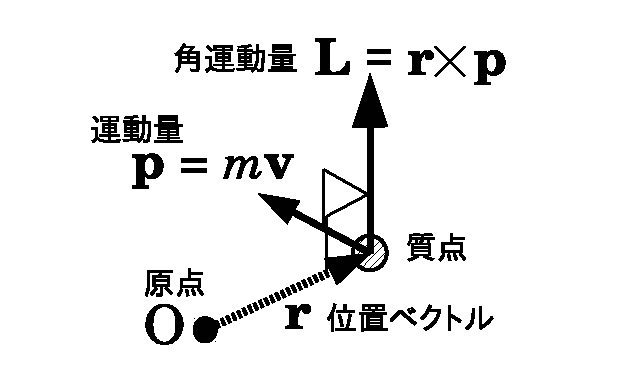
\includegraphics[width=6.5cm]{angular_mom.eps}
    \caption{角運動量の定義。$m$は質点の質量, ${\bf v}$は
質点の速度, ${\bf r}$は質点の位置ベクトル。
${\bf r}, {\bf v}, {\bf p}, {\bf L}$はいずれもベクトル(だから太字)。
$m$はスカラー(だから細字)。}\label{fig:angular_mom}
\end{figure}

\begin{freqmiss}{\small\textgt{${\bf L}={\bf p}\times{\bf r}$と
覚えてしまう} ... ダメです。外積は順序が逆になると結果が異なる
(向きが逆になる)ので, ${\bf p}\times{\bf r}$と${\bf r}\times{\bf p}$
は違います。}\end{freqmiss}

%
\begin{q}\label{q:angular_momentum} 角運動量の定義を確認しよう。
\begin{enumerate} 
\item 角運動量とは何か?
\item 角運動量のSI単位は?
\item 角運動量は, 位置ベクトルと運動量の両方に垂直であることを示せ。
\end{enumerate}
\end{q}
\mv

この「角運動量」なる奇妙な物理量がどのように便利なのかは後回しに
して, とりあえずいくつかの系の角運動量を考えてみることで角運動量に
慣れよう。\mv

%
\begin{q}\label{q:circle_angularmom}
3次元空間に, 座標軸($x,y,z$軸; 各軸は互いに直交している)を設定する。
$xy$平面上で, 原点を中心とする半径$r$の円周上を, 質量$m$の質点が
角速度$\omega$で等速円運動している。時刻$t=0$で質点は$x$軸上にある。
\begin{enumerate}
\item 時刻$t$のときの質点の位置ベクトル${\bf r}$は次式になることを示せ。
\begin{eqnarray}
{\bf r}=r(\cos \omega t, \sin \omega t, 0)\label{eq:circle_angularmom1}
\end{eqnarray}
(ただし, これと逆向きの回転のことは考えないとしよう。)
\item 時刻$t$のときの質点の運動量${\bf p}$は次式になることを示せ。
\begin{eqnarray}
{\bf p}=mr\omega(-\sin \omega t, \cos \omega t, 0)\label{eq:circle_angularmom2}
\end{eqnarray}
\item この質点の角運動量${\bf L}$は次式になることを示し, 時刻$t$によらず
一定値であることを確認せよ(図\ref{fig:angular_mom_circ}参照)。
\begin{eqnarray}
{\bf L}=(0, 0, mr^2\omega)\label{eq:circle_angularmom3}
\end{eqnarray}
\end{enumerate}
\begin{figure}[h]
    \centering
    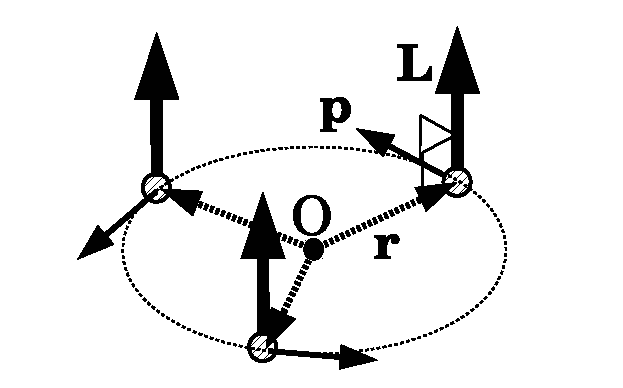
\includegraphics[width=5cm]{angular_mom_circ.eps}
    \caption{等速円運動する質点の角運動量}\label{fig:angular_mom_circ}
\end{figure}\end{q}

この問題の結果から, 原点を中心とする等速円運動をする質点の角運動量は, 
時刻によらず一定であることがわかった。

ちなみに角運動量は, 回転以外の運動についても考えることができる。そもそも, 
角運動量の定義, つまり\eref{eq:def_angmom}には, 運動が回転であるというような
前提は存在しない。\mv

%
\begin{q}\label{q:straight_angularmom}
$xyz$空間の中で, 質量$m$の質点が, 時刻$t$のときに位置ベクトル${\bf r}=(Vt, y_0, 0)$の
位置にいるとしよう。$V$と$y_0$は定数である。
\begin{enumerate}
\item この質点の速度${\bf v}$を求め, この運動が等速直線運動であることを示せ。
\item この質点の運動量${\bf p}$を求めよ。
\item この質点の角運動量${\bf L}$は次式のようになることを示し, 時刻$t$に
よらず一定値であることを確認せよ(図\ref{fig:angular_mom_lin}参照)。
\begin{eqnarray}
{\bf L}=(0, 0, -mVy_0)\label{eq:straight_angularmom}
\end{eqnarray}
\end{enumerate}
\begin{figure}[h]
    \centering
    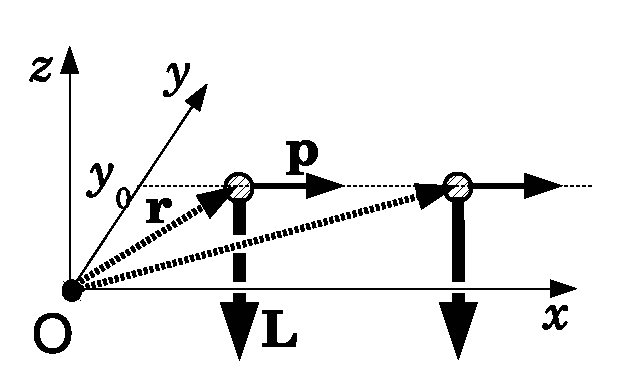
\includegraphics[width=5cm]{angular_mom_lin.eps}
    \caption{等速直線運動する質点の角運動量}\label{fig:angular_mom_lin}
\end{figure}
\end{q}

この問題の結果から, 等速直線運動をする質点の角運動量は, 時刻によらず一定
であることがわかった。

しかし, ちょっと変な気がしないだろうか? 問\ref{q:straight_angularmom}では, 
\eref{eq:straight_angularmom}のように, 角運動量が, $y_0$に依存した。
$y_0$は, 質点が運動する直線(この場合は$x$軸に平行な直線)が原点からどれだけ離れているかを示す
定数である。ということは, 角運動量は, 同じ運動についても, 原点をどこに置くかで, 違った値を持つのだ。
原点をどこに置くかは人間が勝手に決めることなので, 結局, 角運動量の値は, 人間の恣意的な判断に依存
してしまうのだ!

回転運動などを考えるときは, 原点は回転の中心に置くのが普通だし便利だが, 必ずしも
そうでなければならないという必然性は無い。
ならば原点の置き方によって変わる角運動量って, 何なんだ? 
と思うかもしれない。実は, 角運動量は, その値だけで意味を持つのではなく, 次節に述べる
考え方によって意味を持つのだ。そしてこの考え方は, 原点の選択には依存しないのだ。
つまり, どこに原点を置いてもいいし, その結果として角運動量の値がどのように
変わってもかまわないが, それでもなお, 以下の話は
成り立つのだ
\footnote{これはちょうど, ポテンシャルエネルギーの値が
基準点(原点)のとりかたによって異なる, という事情に似ている。原点のとりかた
によってポテンシャルエネルギーは異なっても, ポテンシャルエネルギーの空間微分
は保存力に一致するし(\eref{eq:F_gradU}), 力学的エネルギー保存則は成り立つ。}。
\hv


\section{角運動量保存則}\index{かくうんどうりょうほぞんそく@角運動量保存則}

\eref{eq:def_angmom}の両辺を, 時刻で微分してみよう。質量$m$を一定とすれば, 
\begin{eqnarray}
\frac{d}{dt}{\bf L}&=&\frac{d}{dt}({\bf r}\times {\bf p})\label{eq:dLdt1}\\
                    &=&\frac{d}{dt}(m{\bf r}\times{\bf v})\label{eq:dLdt2}\\
                    &=&m\frac{d}{dt}({\bf r}\times{\bf v})\label{eq:dLdt3}\\
                    &=&m\Bigl(\frac{d{\bf r}}{dt}\times{\bf v}+{\bf r}\times\frac{d{\bf v}}{dt}\Bigr)\label{eq:dLdt4}\\
                    &=&m{\bf v}\times{\bf v}+m{\bf r}\times\frac{d{\bf v}}{dt}\label{eq:dLdt5}
\end{eqnarray}
ここで, \eref{eq:dLdt3}から\eref{eq:dLdt4}の変形において, \eref{eq:vect_vecprod_diff_phys}の
性質を使った。

\eref{eq:dLdt5}について第1項の${\bf v}\times{\bf v}$は恒等的に${\bf 0}$である(性質5より)。
従って, \eref{eq:dLdt5}は, 
\begin{eqnarray}
m{\bf r}\times\frac{d{\bf v}}{dt}\label{eq:dLdt6}
\end{eqnarray}
となる。さらに, 運動方程式
\begin{eqnarray}
m\frac{d{\bf v}}{dt}={\bf F}
\end{eqnarray}
を使うと(${\bf F}$は質点にかかる力), \eref{eq:dLdt6}は, 
\begin{eqnarray} 
{\bf r}\times{\bf F}
\end{eqnarray} 
となる。従って, \eref{eq:dLdt1}左辺から\eref{eq:dLdt5}に至る方程式は, 結局, 
\begin{eqnarray} 
\frac{d}{dt}{\bf L}={\bf r}\times{\bf F}\label{eq:angmomtorq}
\end{eqnarray} 
となる。この右辺に現れた物理量には特別な名前が付けられている:
\begin{itembox}{トルク(力のモーメント)の定義}
${\bf r}\times{\bf F}$, つまり位置ベクトルと力の外積のことを, 
\underline{トルク}(torque)\index{とるく@トルク}とか
\underline{力のモーメント}\index{ちからのもーめんと@力のモーメント}と呼ぶ。
\end{itembox}

そして, \eref{eq:angmomtorq}が表すのは, 
\begin{itembox}{質点に関する角運動量保存則}
質点の角運動量の, 単位時間あたりの変化は, 質点に働くトルクに等しい。
\end{itembox}
という重要な物理法則である\footnote{ただし, これは導出過程から明らかなように, 運動の
3法則(特に${\bf F}=m{\bf a}$)から派生する法則なので, 基本法則とは言えない。}。\mv

\begin{q}\label{q:derive_1_angmom} \eref{eq:angmomtorq}の導出を再現せよ。\end{q}

この法則を複数の質点に拡張しよう。いま, $n$個の質点が互いに力を及ぼしあいながら
運動する状況を考えよう。$k$番目($k=1, 2, \cdots, n$)の質点のことを「質点$k$」と呼び, 
その質量, 位置, 速度, 角運動量をそれぞれ$m_k$, ${\bf r}_k$, ${\bf v}_k$, ${\bf L}_k$
とする。質点$k$にかかる力${\bf F}_k$は, その他の質点から受ける力(内力)と, それ以外
から受ける力(外力)の和である:
\begin{eqnarray} 
{\bf F}_k={\bf F}_{k1}+{\bf F}_{k2}+\cdots+{\bf F}_{kn}+{\bf F}_{k}^{\text{e}}\label{eq:multiforce}
\end{eqnarray} 
ここで${\bf F}_{k1}$, ${\bf F}_{k2}$, ...は, それぞれ, 質点1が質点$k$に及ぼす力, 
質点2が質点$k$に及ぼす力, ...である。質点$k$が自分自身に及ぼす力は考えなくてよいので, 
${\bf F}_{kk}$は考えなくてよいのだが, ここでは形式的に残しておいて, そのかわり
${\bf F}_{kk}={\bf 0}$としよう。また, ${\bf F}_{k}^{\text{e}}$は, 外力が質点$k$に及ぼす力である。
例として, 図\ref{fig:angular_mom_sys}に, 3個の質点からなる質点系に働く力を示す:

\begin{figure}[h]
    \centering
    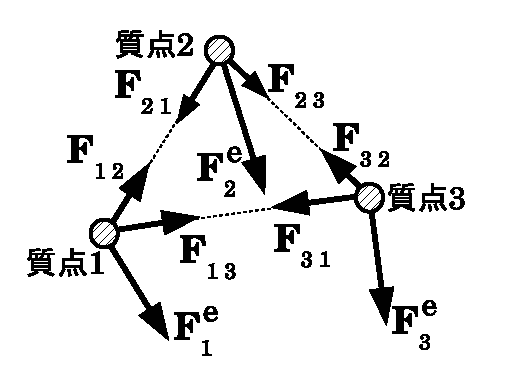
\includegraphics[width=6.0cm]{angular_mom_sys.eps}
    \caption{質点系に働く力。この図では内力どうし(${\bf F}_{12}$と${\bf F}_{21}$など)が
中心力(後述)である(同一直線上にある)ことを仮定している。}\label{fig:angular_mom_sys}
\end{figure}

さて, 質点$k$について, \eref{eq:angmomtorq}, \eref{eq:multiforce}を考えると, 
\begin{eqnarray}\frac{d}{dt}{\bf L}_k={\bf r}_k\times{\bf F}_k\end{eqnarray}
\begin{eqnarray} 
={\bf r}_k\times({\bf F}_{k1}+{\bf F}_{k2}+\cdots+{\bf F}_{kn}+{\bf F}_{k}^{\text{e}})
\end{eqnarray} 
である。同様の式を, 全ての質点に関して考えて, 
\begin{eqnarray*}
&&\frac{d}{dt}{\bf L}_1={\bf r}_1\times({\bf F}_{11}+{\bf F}_{12}+\cdots+{\bf F}_{1n}+{\bf F}_{1}^{\text{e}})\\
&&\frac{d}{dt}{\bf L}_2={\bf r}_2\times({\bf F}_{21}+{\bf F}_{22}+\cdots+{\bf F}_{2n}+{\bf F}_{2}^{\text{e}})\\
&&\cdots\\
&&\frac{d}{dt}{\bf L}_n={\bf r}_n\times({\bf F}_{n1}+{\bf F}_{n2}+\cdots+{\bf F}_{nn}+{\bf F}_{n}^{\text{e}})
\end{eqnarray*}
これらを辺々足し合わせると, 
\begin{eqnarray}
\sum_{k=1}^n \frac{d}{dt}{\bf L}_k
&=&\sum_{k=1}^n{\bf r}_k\times({\bf F}_{k1}+{\bf F}_{k2}+\cdots+{\bf F}_{kn})\nonumber\\
&+&\sum_{k=1}^n{\bf r}_k\times{\bf F}_{k}^{\text{e}}
\label{eq:totangmomtorq0}
\end{eqnarray}
この式の右辺の最初の$\sum$に注目しよう。この和を分解して考えると, その中には, 
1以上$n$以下の任意の$j, k$について($j\ne k$とする), 1つの${\bf r}_j\times{\bf F}_{jk}$
と1つの${\bf r}_k\times{\bf F}_{kj}$が存在する。これらをひとまとめにすると, 
\begin{eqnarray} 
{\bf r}_j\times{\bf F}_{jk}+{\bf r}_k\times{\bf F}_{kj}\label{eq:pairtorq}
\end{eqnarray} 
となる。ところが, 作用反作用の法則から, 
\begin{eqnarray} 
{\bf F}_{kj}=-{\bf F}_{jk}\label{eq:actreact}
\end{eqnarray} 
である。従って, 式(\ref{eq:pairtorq})は, 以下のようになる:
\begin{eqnarray} 
({\bf r}_j-{\bf r}_k)\times{\bf F}_{jk}\label{eq:pairtorq2}
\end{eqnarray} 
${\bf r}_j-{\bf r}_k$は質点$k$から質点$j$へのベクトルである。

ところで, 質点どうしが及ぼし合う力が, 互いを結んだ直線上にある場合, すなわち
互いの方向(もしくは逆方向)をまっすぐに向いているような場合, 
そのような力を\underline{中心力}\index{ちゅうしんりょく@中心力}という\footnote{重力や静電気力(クーロン力)は
中心力である。}。\textgt{もし, ${\bf F}_{kj}$が中心力であると
仮定すれば}, ${\bf r}_j-{\bf r}_k$と${\bf F}_{jk}$は互いに平行だから, 
その外積は${\bf 0}$になる(性質5より)。従って, 
式(\ref{eq:pairtorq2})は恒等的に${\bf 0}$になる。そのことと, ${\bf F}_{kk}={\bf 0}$を使えば, 
式(\ref{eq:totangmomtorq0})は, 右辺の最初の$\sum$が${\bf 0}$になってしまって, 
\begin{eqnarray} 
\sum_{k=1}^n \frac{d}{dt}{\bf L}_k=\sum_{k=1}^n{\bf r}_k\times{\bf F}_{k}^{\text{e}}
\end{eqnarray} 
となる。ここで左辺の$t$による微分を$\sum$の前に出せば, 
\begin{eqnarray} 
\frac{d}{dt}\sum_{k=1}^n {\bf L}_k=\sum_{k=1}^n{\bf r}_k\times{\bf F}_{k}^{\text{e}}\label{eq:totangmomtorq1}
\end{eqnarray} 
となる。この式は味わい深い。左辺の$\sum$は全質点の角運動量の和であり, 
全角運動量という。右辺は, 各質点に働く外力によるトルクの和だ。すなわち, 以下の法則が成り立つことが証明された:
\begin{itembox}{質点系に関する角運動量保存則(1)}
内力が中心力であるような質点系(質点の集合)については, その全角運動量の, 
単位時間あたりの変化は, 各質点に働く外力によるトルクの総和に等しい。
\end{itembox}

\begin{q}\label{q:derive_n_angmom} \eref{eq:totangmomtorq1}の導出を再現せよ。\end{q}

ここで, \textgt{特に, 全ての質点が静止していれば}, 当然ながら全ての$k$
について${\bf L}_k={\bf 0}$が恒等的に成り立つ。従って, 
そのとき全角運動量$\sum_{k=1}^n{\bf L}_k$も恒等的に${\bf 0}$である。従って, それを
$t$で微分したもの(\eref{eq:totangmomtorq1}の左辺)も恒等的に${\bf 0}$である。
従って, \eref{eq:totangmomtorq1}の右辺も恒等的に${\bf 0}$である:
\begin{eqnarray} 
\sum_{k=1}^n{\bf r}_k\times{\bf F}_{k}^{\text{e}}={\bf 0}\label{eq:totangmomtorq2}
\end{eqnarray} 
この式の意味するのは, 「\textgt{内力が中心力であり, 静止状態にある質点の集まりでは, 
外力によるトルクの和は${\bf 0}$}」ということだ。物体とは無数の原子や電子(質点と考えられる)
の集まりなので, 上の文章の「質点の集まり」は「物体」であっても差し支えない。
これが物体の静止状態における, 「(力の)\underline{モーメントのつりあい}」
\index{もーめんとのつりあい@モーメントのつりあい}である。
その特別な場合が「てこの原理」だ。第3章では, 仮想仕事の原理から「てこの原理」
つまり\eref{eq:principle_balance}を導いたが, このように, 
運動方程式から導くこともできるのだ\footnote{力学の法則は
全て運動の法則から導かれるという立場からすると, これはむしろ自然
である。不思議なのは, 仮想仕事の原理という考え方から出発しても, 
同じ結論が導かれたことである。}。\mv

さて, \eref{eq:totangmomtorq1}に戻ろう。こんどは, 質点は静止していない(運動している)が, 
\textgt{外力は働かない}(内力は中心力だけが働く)ような状況を考えよう。
その場合, \eref{eq:totangmomtorq1}の右辺は${\bf 0}$だ。従って, 
\begin{eqnarray} 
\frac{d}{dt}\sum_{k=1}^n {\bf L}_k={\bf 0}\label{eq:totangmomtorq3}
\end{eqnarray} 
である。この式は, 全角運動量は時刻$t$によらず一定である, ということだ。従って, 
次の法則が成り立つことがわかった:
\begin{itembox}{質点系に関する角運動量保存則(2)}
外力が無く, 内力が中心力である場合は, 全角運動量は時刻によらず一定である。
\end{itembox}


%
\begin{q}\label{q:torque} 
\begin{enumerate}
\item トルクとは何か? 
\item トルクは, 別名, 何というか? 
\item トルクのSI単位は? 
\item 中心力とは何か? 
\item モーメントのつりあいとは何か? 
\item 角運動量保存則とは何か? 
\end{enumerate}
\end{q}
\vspace{0.2cm}

%
\begin{q}\label{q:2points_rotation}
質量$m$の質点が2つあって, 伸縮可能な軽い棒でつながっている。棒の長さを$2r$としよう。
さて最初は, 棒の長さが一定で, 2つの質点は棒の真ん中を中心とする等速円運動をしている。
そのときの角速度を$\omega$とする。なお, 中心は静止している。質点どうしに働く力は
中心力であるとする。
\begin{enumerate}
\item 1つの質点の運動量${\bf p}$の大きさ$|{\bf p}|$は, $mr\omega$であることを示せ。
\item 1つの質点の角運動量${\bf L}$の大きさ$|{\bf L}|$は, $mr^2\omega$であることを示せ。
\item それぞれの質点の角運動量は, どのような方向を向いているか? 
\item 全角運動量の大きさは$2mr^2\omega$であることを示せ。
\item 全運動エネルギー(各質点の運動エネルギーの和)$T$は$T=mr^2\omega^2$であることを示せ。
\item ある時点で, 棒が急に縮んで長さが半分になったとする。角速度はどうなるか? 
\item そのとき, 運動エネルギーはどうなるか? 
\item 棒が縮む前と後で運動エネルギーが違うが, それはエネルギー保存則と矛盾しないのだろうか? 
\end{enumerate}
\end{q}
\hv


\section{解答}

\noindent{\textbf{答}}\ref{q:univ_vectprod0_phys} 略(「大学1年生のための数学入門」に同じ問題が載っているので。)\\

\noindent{\textbf{答}}\ref{q:vect_vecprod_diff_phys} 略(「大学1年生のための数学入門」に同じ問題が載っているので。)\\

% 角運動量とは何か? 角運動量の次元は? 
\noindent{\textbf{答}}\ref{q:angular_momentum} 
(1) 略。
(2) ${\bf r}$のSI単位はm, ${\bf p}$のSI単位はkg~m~s$^{-1}$。従って, ${\bf r}\times{\bf p}$
のSI単位はkg~m$^2$~s$^{-1}$。注: 外積は単なる「積」ではないが, その定義を見れば, 2つの物理量の
外積の単位は, 元の物理量の単位の積になることがわかるだろう。
(3) 外積の性質2より, ${\bf r}\times{\bf p}$は${\bf r}$と${\bf p}$の両方に垂直。
\mv

% $xyz$空間の中の$xy$平面上で, 原点を中心とする半径$r$の円周上を
\noindent{\textbf{答}}\ref{q:circle_angularmom}
(1) 題意より, 質点の位置は$xy$平面に限定されるので, $z$座標は常に0である。また, $xy$平面
内では, 原点から距離$r$で$x$軸から角度$\omega t$だけ回転した位置に質点はあるので, その位置
は\eref{eq:circle_angularmom1}のようになる。
(2) \eref{eq:circle_angularmom1}を$t$で微分すると速度になる。それに$m$をかければ
与式を得る。
(3) ${\bf L}={\bf r}\times{\bf p}$
\begin{eqnarray*}
&=&mr^2\omega(\cos \omega t, \sin \omega t, 0)
      \times(-\sin \omega t, \cos \omega t, 0)\\
&=&(0, 0, mr^2\omega)
\end{eqnarray*}
これは$t$を含まない式なので, $t$によらず一定。
\mv

% $xyz$空間の中で, 質量$m$の質点が, 時刻$t$のときに位置ベクトル
\noindent{\textbf{答}}\ref{q:straight_angularmom}
(1)
\begin{eqnarray*}\frac{d}{dt}{\bf r}=\frac{d}{dt}(Vt,\, y_0,\, 0)=(V,\, 0,\, 0)\end{eqnarray*}
この式は, この質点が$x$軸方向に一定の速度で運動することを示している。従って等速直線運動。
(2) ${\bf p}=m{\bf v}=(mV, 0, 0)$。
(3) ${\bf L}={\bf r}\times{\bf p}=(Vt,\, y_0,\, 0)\times(mV,\, 0,\, 0)
       =(0,\, 0,\, -mVy_0)$。
これは$t$を含まない式なので, $t$によらず一定。
\mv

% トルクとは何か? トルクは,
\noindent{\textbf{答}}\ref{q:torque} 略。トルクのSI単位はN~m=kg~m$^2$s$^{-2}$。
なんと, これはJ, すなわちエネルギーの単位ではないか! しかし, 書き方の慣習
として, トルクはJで書くことはほとんどなく, N~mで書くことの方が圧倒的に多い。
もちろんJとN~mは本質的に全く同じ単位なのだが, あくまで慣習としてである。
\vspace{0.2cm}

% 質量$m$の質点が2つあって, 伸縮可能な軽い棒でつながっている。
\noindent{\textbf{答}}\ref{q:2points_rotation}
適当に座標をとれば, 1つの質点の位置は
${\bf r}=(r\cos\omega t, r\sin\omega t, 0)$と書ける。
\begin{enumerate}
\item ${\bf p}=m{\bf r}'=m(-r\omega\sin\omega t, r\omega\cos\omega t, 0)$
従って, $|{\bf p}|=mr\omega$。
\item ${\bf L}={\bf r}\times{\bf p}$
\begin{eqnarray*}
  &=&(r\cos\omega t, r\sin\omega t, 0)\times m(-r\omega\sin\omega t, r\omega\cos\omega t, 0)\\
  &=&mr^2\omega(\cos\omega t, \sin\omega t, 0)\times (-\sin\omega t, \cos\omega t, 0)\\
  &=&mr^2\omega(0, 0, \cos^2\omega t+\sin^2\omega t)\\
  &=&mr^2\omega(0, 0, 1)
\end{eqnarray*}
従って, $|{\bf L}|=mr^2\omega$
\item ともに$z$軸の正方向を向いている。
\item 小問(2)の解答より, 2つの質点は, 同じ大きさで同じ向きの角運動量を持っている。従って, 
全角運動量の大きさは, 1つの質点の角運動量の2倍, すなわち$2mr^2\omega$である。
\item 1つの質点の運動エネルギーは, 
\begin{eqnarray*}\frac{1}{2}mv^2=\frac{1}{2}m(r\omega)^2=\frac{mr^2\omega^2}{2}\end{eqnarray*}
である。全質点の運動エネルギーは, この2倍なので, $T=mr^2\omega^2$となる。
\item 縮んだ後の角速度を$\Omega$とすると, 小問(4)と同様に考えれば, 
縮んだ後の全角運動量の大きさは
\begin{eqnarray*}2m\Bigl(\frac{r}{2}\Bigr)^2\Omega\end{eqnarray*}
である。質点系の角運動量保存則より, これは縮む前の全角運動量の大きさに等しいはず
(もちろん全角運動量の方向も変わらないはずだが, ここではそれを使う必要はない)。
従って, 
\begin{eqnarray*}2mr^2\omega=2m\Bigl(\frac{r}{2}\Bigr)^2\Omega\end{eqnarray*}
従って, $\Omega=4\omega$。すなわち, 角速度は4倍になる。
\item 縮んだ後の運動エネルギーは, 小問(5)と同様に考えて
\begin{eqnarray*}
m\Bigl(\frac{r}{2}\Bigr)^2\Omega^2
=m\Bigl(\frac{r}{2}\Bigr)^2(4\omega)^2
=4mr^2\omega^2
\end{eqnarray*}
すなわち, 運動エネルギーは4倍になる。
\item エネルギー保存則によれば, 物体の運動エネルギーは, なされた仕事のぶんだけ
増加する。この場合も, 運動エネルギーが増加しているが, それは, 棒が縮む際に, 2つの
質点どうしを近づけるために力が必要だったのであり, その力がなした仕事が, 2つの質点の
回転に関する運動エネルギーを増加させたのである。
\end{enumerate}
\hv




\section{補遺: 熱放射}\label{sect:thermalemission}\index{ねつほうしゃ@熱放射}

我々の身の回りは, 光に満ち溢れているが, その光はどこでどのように発生する
のだろうか? 例えば太陽, 白熱電球, 蛍光灯, レーザー, 発光ダイオードなどの
光源はどのような仕組みで光るのだろうか?

物体を構成する分子や原子は, 前述したように固有エネルギーを持つ。
そのエネルギーとは, もとをたどれば, 分子・原子・電子等の持つ運動エネルギーや
ポテンシャルエネルギーだ。

固有エネルギーは, 低いものから高いものまで, 離散的に(階段状に)存在
する。それらをエネルギー準位と呼ぶ。そして, 個々の分子や原子のエネルギーが, 
高い順位から低い順位に移り変わることがある。これを「遷移」\index{せんい@遷移}
と言う。原子や分子が遷移するとき, そのエネルギーの差は, 何らかの形で
原子や分子から放出される(でなければエネルギー保存則が成り立たない)。
その「何らかの形」のひとつとして光を出すのが, 蛍光灯, レーザー, 
発光ダイオード等だ。

太陽や白熱電球も, 結局はそのような仕組みで光るのだが, 他とはちょっと違う。太陽や白熱電球
は, 「熱が光に転化する」という仕組みで光るのだ。

先述のように, 物体を構成する粒子は, その温度に応じたエネルギーを, 平均的に持つ。「平均的」
ということは, 実際にはそれよりも大きなエネルギーを持つ粒子も多少あれば, それよりも小さな
エネルギーを持つ粒子も多少はある。その状況で, 粒子が遷移すると, 光が放出され, 粒子の
エネルギーは若干下がる。そしてエネルギーが下がった粒子は周囲の粒子と衝突したり光を
吸収したりして, 再びもとのエネルギーに戻る。このようなことが無数に発生することで, 
その物体から光が出続けるのだ。このような仕組みを「熱放射」と呼ぶ。

実は, 太陽や白熱電球だけでなく, ほとんど全ての物体は, \underline{それぞれの温度に応じて熱放射
している}。例えば, 君の体も熱放射している。君の体も光っているのだ!! ただし, 
その光は, 人の肉眼で見える光(可視光)ではなく, 赤外線だ。だから, 赤外線を検知
できるセンサーで人体を調べれば, 君の体表面の温度がわかるのだ。赤外線体温計
はそれを利用している。また, 夜行性の動物を観察するのに赤外線カメラというものをよく
使う(NHKの番組「ダーウィンが来た!」を見よ)。が, それも同じ事だ。
動物は体温が高いため, 周囲よりも多くの赤外線を出す。それを検出するのだ。

%熱放射の仕組みを定量的にきちんと理解するには, 量子統計力学という
%物理学を学ばねばならない(それは大学3年生のレベルである)。ここでは, 
%以上のような定性的な説明を受け入れて欲しい。

%熱放射を
%説明するのは, 以下の「プランクの法則」である:
%\begin{itembox}{プランクの法則}
%\begin{eqnarray}
%B_{\lambda}(T)=\frac{2\pi h c^2}{\lambda^5}\frac{1}{\exp(\frac{hc}{\lambda k_{\text{B}}T})-1}
%\end{eqnarray}
%絶対温度$T$の完全黒体から放射する光のエネルギーは, 

